\documentclass[]{report}
\usepackage[utf8]{inputenc}
\usepackage{hyperref}
\usepackage{amsmath}
\usepackage{bera}
\usepackage{listings}
\usepackage{xcolor}
\usepackage{graphicx}
\usepackage{placeins}
\usepackage{tikz}
\usetikzlibrary{positioning}

\tikzset{%
  every neuron/.style={
    circle,
    draw,
    minimum size=1cm
  },
  neuron missing/.style={
    draw=none, 
    scale=4,
    text height=0.333cm,
    execute at begin node=\color{black}$\vdots$
  },
}

\graphicspath{{../../figures/}}

\title{
    {Moral AI IQP}\\
    {\large Worcester Polytechnic Institute}\\
    {
\includegraphics[height=2in]{figures/WPI_Inst_Prim_FulClr.png}}
}
\author{Ryan Benasutti}
\date{April 2019}

\newcommand{\code}{\texttt}

\begin{document}

\maketitle

\clearpage
\mbox{}
\clearpage

\chapter*{Abstract}

Artificial intelligence is being deployed in increasingly autonomous systems where it will have to
make moral decisions. However, the rapid growth in artificial intelligence is outpacing the research
in building explainable systems. In this paper, a number of problems around one facet of explainable
artificial intelligence, training data, is explored. Possible solutions to these problems are
presented. Additionally, the human decision-making process in unavoidable accident scenarios is
explored through qualitative analysis of survey results.

\chapter*{Acknowledgements}

\begin{enumerate}
    \item Professor Therese Smith
    \item Professor Yunus Telliel
    \item Griffin Tabor
\end{enumerate}

\tableofcontents

\FloatBarrier
\chapter{Introduction}

This work has two primary goals. First, we seek to demonstrate how a neural network can learn a bias
and empirically determine the severity of that bias. Classification accuracy testing will be
employed to evaluate the trained neural network and determine if any bias was learned, and, if so,
the severity of that bias. Second, we also seek to understand the decision-making process in humans
behind making moral decisions in unavoidable accident scenarios, i.e., dilemmas. This part of the
research will be done by surveying a group of people and performing qualitative analysis on the
survey results. These results serve not only as a way to understand this decision-making process but
also as a language and structure we can use to craft communications with those unfamiliar with
artificial intelligence.

Chapter two provides an overview of what explainable AI is and the current demands for it, in
addition to covering prior research into how humans think when presented with a dilemma. Chapter
three discusses the architecture, training, and testing of a neural network and what questions we
asked in the aforementioned survey. Chapter four analyses the neural network testing results and the
survey results. Chapter five concludes this work and provides avenues for future inquiry.


\FloatBarrier
\chapter{Background}

Introduce background readings (maybe not first?).

Autonomous vehicle technology is growing rapidly and AI is a key piece of that technology. As this
technology gets closer to attaining full autonomy, the AI deployed in these systems will have
greater responsibility than ever. These AI systems must be explainably fair, i.e., they must both
make decisions using only the least amount of information necessary for optimal performance and make
those decisions predictably and correctly. For example, the AI in an autonomous vehicle does not
need to be supplied with information about a pedestrian's race, even though race may be an impactful
trait in other fields, especially medical fields~\cite{sickeCellDisease}. Furthermore, these AI
systems must also be explainable for legal reasons, such as determining which party is at fault in
the event of a car accident or, in the European Union, complying with a user's "right to
explanation"~\cite{goodman2017european}.

The demand for explainable AI is increasing, as illustrated by DARPA's Explainable Artificial
Intelligence (XAI) program~\cite{gunning2016explainable}. This program aims to develop explainable
AI systems such as in Figure~\ref{fig:darpa_xai}. There has also been a symposium focusing on AI
inclusivity towards marginalized peoples~\cite{berkmanKleinCenterAI2017,aiAndInclusionSymposium}.
This symposium illustrates the increasing need to discuss AI fairness and inclusivity in a way that
non-technical people can understand. One facet of this need that this paper addresses is the
question of specifically how much one needs to care about possible biases in the various stages of
AI architecture. Not all AI research involving morally responsible AI systems has a focus on
explainability, however. NVIDIA trained an end-to-end convolutional neural network, which "[maps]
raw pixels from a single front-facing camera directly to steering commands" \cite{bojarski2016end}.
With this approach, the AI will have to respond directly to pedestrians and other external stimuli.

\begin{figure}[h]
    \centering
    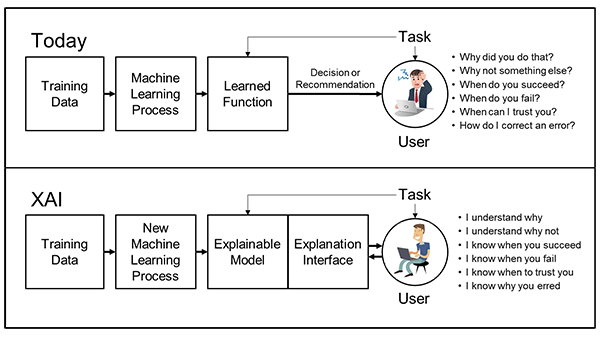
\includegraphics[scale=1.1]{figures/xai-figure2.png}
    \caption[]{DARPA's XAI Concept~\protect\cite{gunningXAIProgram}}
    \label{fig:darpa_xai}
\end{figure}

We must also address the ethical and moral side of AI. A reflection on ethics is critical to avoid
building irresponsible AI systems. These systems affect, or will affect in the near future, many
people's lives. Take, for example, the case of an autonomous vehicle. By allowing autonomous
vehicles in our society, we are accepting the dangers they bring in exchange for the benefits they
provide; among these dangers are injury and loss of life to those involved in vehicular accidents.
Those developing AI systems therefore have a responsibility to improve these systems and reduce the
dangers associated with their use. They also have a responsibility to "assess, and try to inform
others of, the possible social consequences" of these systems~\cite{patrick2017robot}. We can then
conclude that building AI systems carries with it moral responsibility. This realization can also be
seen in a proposed bill, the "Algorithmic Accountability Act of 2019" by Senator Wyden, which would
have the Federal Trade Commission "create regulations requiring companies under its jurisdiction to
conduct impact assessments of highly sensitive automated decision systems", require companies
"assess their use of automated decision systems", and require companies "correct any issues they
discover during the impact assessments"~\cite{wyden2019bill}. This bill is effectively an effort to
extend anti-discrimination laws to "automated decision systems", which, as of late, are typically AI
systems.

The software architects, engineers, and researchers which build AI systems must address moral
concerns about explainability and fairness in their products. However, they may be morally uncertain
with respect to how they can address these concerns. Resolving this moral uncertainty is a
nontrivial problem. Simply choosing a resolving act based on personal preference is clearly
unacceptable. A "Continue Deliberating" strategy is equivalent to an instance of the previous
strategy, so it is also unacceptable~\cite{patrick2017robot}. An ethical framework, then, is
required to resolve this uncertainty. The work of Bhargava and Kim \cite{patrick2017robot} proposes
an "Expected Moral Value" approach which acts as an ethical meta-framework one can use to resolve
this moral uncertainty. While this cannot act as a universal solution, it shows progress in the
right direction and serves as a starting point of inquiry for those building AI systems.

Moving to the domain of how humans think about dilemmas, we look towards the Moral Machine
experiment~\cite{awad2018moral}, which is prior research into people's preferences in moral
dilemmas. This experiment involved an online survey in which participants are shown a moral dilemma
involving an autonomous vehicle, passengers, and pedestrians. In each dilemma, the participant must
choose between inaction, which typically results in the certain death of the pedestrians, and
action, which typically results in the certain death of the passengers. The study revealed three
strong global preferences towards sparing humans over animals, sparing more lives rather than fewer,
and sparing younger lives rather than older. The study also showed that some preferences vary
between countries depending on that country's propensity towards egalitarianism.

\FloatBarrier
\chapter{Methods}

\section{Data Generation}

The data is generated using a graphical model to control the conditional probabilities for the
states of each variable. The variables in the model correspond directly to the attributes of a
person. Figure~\ref{fig:graphical_model_image} is a rendering of the graphical model. For example,
people in the first option could be more likely to jaywalk than people in the second option,
producing a data set which is biased towards/against jaywalkers. When combined with control over the
number of people in each option, this method can produce both subtle and strong bias. The code for
the domain of each attribute of a person is in Figure~\ref{fig:code_for_person_attribute_domains}.
The Python library \href{https://github.com/pgmpy/pgmpy}{pgmpy} is used to create the graphical
model and infer each variable’s probability distribution. These distributions are then used to pick
elements from each variable’s domain. This process is repeated for each attribute of each person and
for the number of people in each option of a dilemma, forming a complete dilemma. The number of
dilemmas generated is specified programmatically using the \code{TrainMetadata} class, which
captures the number of dilemmas to generate and the maximum number of people per option.

\begin{figure}[h]
    \centering
    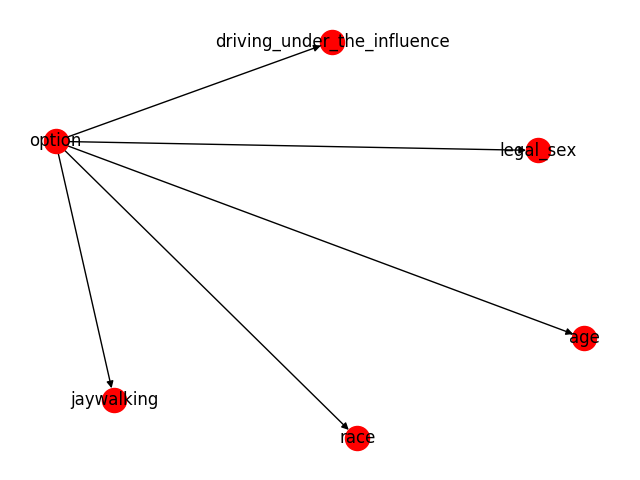
\includegraphics[scale=0.6]{figures/network.png}
    \caption[]{The graphical model.}
    \label{fig:graphical_model_image}
\end{figure}

\begin{figure}[h]
    \centering
    \begin{verbatim}
    age_states = [10, 20, 30, 40, 50, 60]
    race_states = [Race.white, Race.black, Race.asian,
                Race.native_american, Race.other_race]
    legal_sex_states = [LegalSex.male, LegalSex.female]
    jaywalking_states = [False, True]
    driving_under_the_influence_states = [False, True]
    \end{verbatim}
    \caption{Python code for the bracketed attributes of a Person}
    \label{fig:code_for_person_attribute_domains}
\end{figure}

\FloatBarrier
\section{Data Bracketing}
\label{sec:data-bracketing}

Attributes are one-hot encoded (i.e., mapped using an indicator function) so the neural network is
resilient to unspecified attributes. Age is bracketed by increments of 10 years. Some example
encoded ages are shown in Table~\ref{tab:example_age_attribute_encoding}. Boolean attributes are
encoded into three increments, as shown in Table~\ref{tab:example_boolean_attribute_encoding}.
    
\begin{table}[h]
    \centering
    \begin{tabular}{c|c|c|c|c|c|c|c}
        Age (yr) & unspecified & 1-10 & 11-20 & 21-30 & 31-40 & 41-50 & 51-60 \\\hline
        unspecified & 1 & 0 & 0 & 0 & 0 & 0 & 0 \\
        0 & 0 & 1 & 0 & 0 & 0 & 0 & 0 \\
        3 & 0 & 1 & 0 & 0 & 0 & 0 & 0 \\
        16 & 0 & 0 & 1 & 0 & 0 & 0 & 0 \\
        42 & 0 & 0 & 0 & 0 & 0 & 1 & 0
    \end{tabular}
    \caption{Example age attribute encoding.}
    \label{tab:example_age_attribute_encoding}
\end{table}

\begin{table}[h]
    \centering
    \begin{tabular}{c|c|c|c}
        Value & unspecified & false & true \\\hline
        unspecified & 1 & 0 & 0 \\
        false & 0 & 1 & 0 \\
        true & 0 & 0 & 1
    \end{tabular}
    \caption{Example boolean attribute encoding.}
    \label{tab:example_boolean_attribute_encoding}
\end{table}

\FloatBarrier
\section{Data Storage}

Data is stored using the JSON format using a serialization process called pickling via the Python
library \href{https://jsonpickle.github.io/}{jsonpickle}. This process was chosen because it
produces easily machine-readable files and because JSON is a popular data storage format. The
purpose of storing the generated data sets is to keep the data consistent between test iterations
and to share the data. Both the training and test data sets are pickled after generation.

\FloatBarrier
\section{Neural Network Model}

There are two primary requirements of the neural network used in the experiments. First, the network
must classify the training data. In other words, when given a dilemma, the network must classify
that dilemma by picking which option to avoid. For example, in a dilemma with two options of three
and four people, respectively, the correct classification is the second option because it allows the
autonomous vehicle to save more people. In the case where a dilemma has two or more options of equal
size, the earlier option is chosen.

Second, the network must be easy to train, meaning that the time required to train the network must
be small (on the order of minutes or less) and the hardware resources required to train the network
must be minor. Testing the network requires training it many times, so the time required to train
the network must be small. Additionally, the network will be trained on personal machines, so any
hardware requirements must be easy to meet.

There are three models which were considered when deciding on what network to use. First, an
autoencoder: autoencoders are trained using unsupervised learning, so labeling the data is not
necessary (want to avoid imparting a set of morals). This model would perform dimensionality
reduction, and perhaps learn to ignore noise (i.e., uniformly distributed attributes) in the data
set, but would be unable to classify the dilemmas.

Second, an autoencoder in combination with a simple neural network trained using supervised
learning: this model solves the classification problem which the previous model failed at, but
introduces unnecessary complexity to the research. The intent of this research is not to build a
neural network capable of guiding a real autonomous vehicle, so this model was deemed unnecessarily
complex.

Lastly, a recurrent neural network (RNN) with long short-term memory (LSTM). This option was
considered because RNN's are capable of accepting variable-length sequential data. We thought the
network may need to handle variable-length data, but the engineering challenge that design posed was
traded in favor of both limiting the maximum number of people in an option and bracketing the data
as covered in section~\ref{sec:data-bracketing}. Additionally, this network does not directly solve
the classification problem, so it is only marginally applicable for this research.

The final neural network chosen is a simple, shallow, feed-forward network with one hidden layer
trained using supervised learning, pictured in Figure~\ref{fig:shallow_neural_network}. The input
layer has dimensionality equal to the number of attributes per person (after one-hot encoding)
multiplied by the number of options per dilemma multiplied by the maximum number of people per
option. The output layer has dimensionality equal to the number of options per dilemma. The hidden
layer has dimensionality equal to the average of that of the input and output layers. An example
implementation in Keras of the model can be seen in Figure~\ref{fig:code_for_model}.

\begin{figure}[h]
    \centering
    
    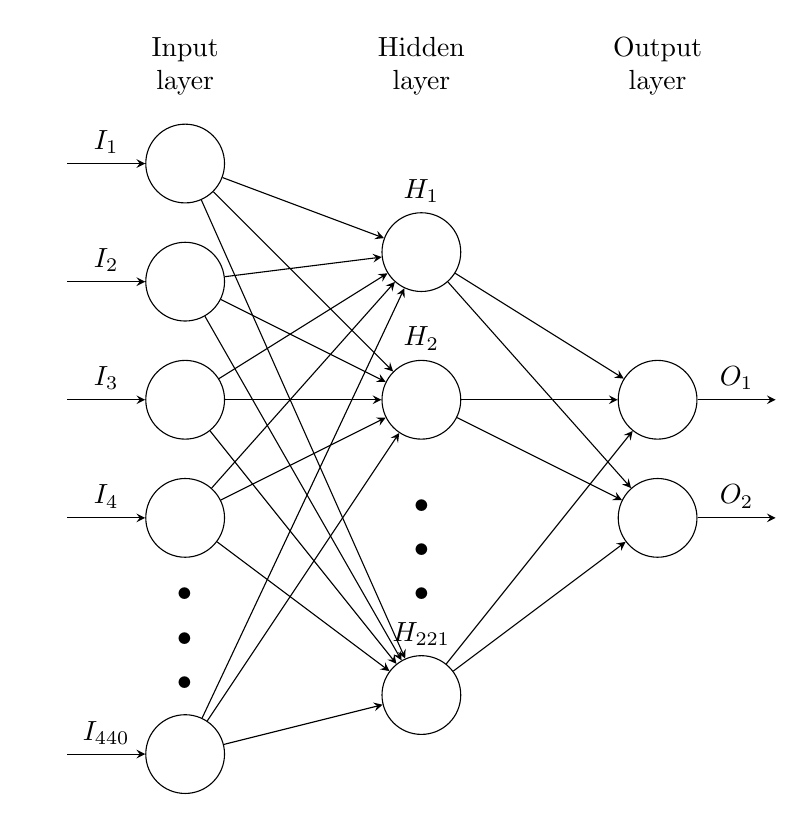
\begin{tikzpicture}[x=1.5cm, y=1.5cm, >=stealth]
        \foreach \m/\l [count=\y] in {1,2,3,4,missing,5}
          \node [every neuron/.try, neuron \m/.try] (input-\m) at (0,2.5-\y) {};
        
        \foreach \m [count=\y] in {1,2,missing,3}
          \node [every neuron/.try, neuron \m/.try ] (hidden-\m) at (2,2-\y*1.25) {};
        
        \foreach \m [count=\y] in {1,2}
          \node [every neuron/.try, neuron \m/.try ] (output-\m) at (4,0.5-\y) {};
        
        \foreach \l [count=\i] in {1,2,3,4,\text{440}}
          \draw [<-] (input-\i) -- ++(-1,0)
            node [above, midway] {$I_\l$};
        
        \foreach \l [count=\i] in {1,2,\text{221}}
          \node [above] at (hidden-\i.north) {$H_\l$};
        
        \foreach \l [count=\i] in {1,2}
          \draw [->] (output-\i) -- ++(1,0)
            node [above, midway] {$O_\l$};
        
        \foreach \i in {1,...,5}
          \foreach \j in {1,...,3}
            \draw [->] (input-\i) -- (hidden-\j);
        
        \foreach \i in {1,...,3}
          \foreach \j in {1,...,2}
            \draw [->] (hidden-\i) -- (output-\j);
        
        \foreach \l [count=\x from 0] in {Input, Hidden, Output}
          \node [align=center, above] at (\x*2,2) {\l \\ layer};
        \end{tikzpicture}
    
    \caption[]{A shallow feed-forward neural network with one hidden layer.}
    \label{fig:shallow_neural_network}
\end{figure}

\begin{figure}[h]
    \centering
    \begin{verbatim}
    output_dim = 2
    input_dim = 22 * output_dim * \
            train_metadata.max_num_people_per_option

    model.add(Dense(units=input_dim, activation='relu',
                input_dim=input_dim))
    model.add(Dense(units=round((input_dim + output_dim) / 2),
                activation='relu'))
    model.add(Dense(units=output_dim, activation='softmax'))
    \end{verbatim}
    \caption{The Keras code for the neural network model.}
    \label{fig:code_for_model}
\end{figure}

\FloatBarrier
\section{Neural Network Training}

The training data given to the network is categorical, so the categorical cross entropy loss
function is used. As the network is quite simple, a stochastic gradient descent optimizer suffices.
Training happens over $5$ epochs with a batch size of $32$. An example implementation in Keras can
be seen in Figure~\ref{fig:code_for_training}; additionally, Figure~\ref{fig:neural_network_model}
provides a simple visualization of the dimensionality of the network.

\begin{figure}[h]
    \centering
    \begin{verbatim}
    model.compile(loss=losses.categorical_crossentropy,
                  optimizer='sgd',
                  metrics=[metrics.categorical_accuracy])
    
    model.fit(train_data, train_labels, epochs=5, batch_size=32)
    \end{verbatim}
    \caption{The Keras code for the neural network model.}
    \label{fig:code_for_training}
\end{figure}

\begin{figure}[h]
    \centering
    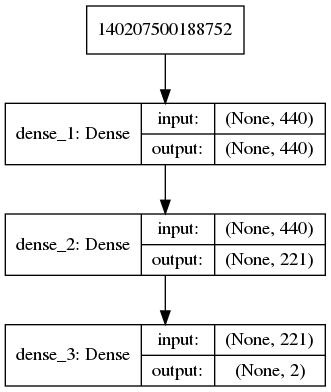
\includegraphics[scale=0.5]{figures/neural_network_model.png}
    \caption[]{The dimensions of the neural network used in this research.}
    \label{fig:neural_network_model}
\end{figure}

\FloatBarrier
\section{Neural Network Testing}

The neural network is tested using Keras to evaluate the classification accuracy and loss against a
test data set. The test data is generated using a graphical model in the same manner as the training
data; however, it is important to note that in this step, the test data is generated separately from
the training data: it is not a sampled subset of the training data. Each training data set is tested
five times. Each iteration involves training the neural network on the training data set and
evaluating its performance against a test data set to collect classification accuracy and loss
information. The results of all five iterations are averaged to produce an average classification
accuracy and loss. Many training data sets are generated and tested against the same test data set.
Each data point in Figure~\ref{fig:test_40-60_100-0_0-100_accuracy_plot} corresponds to a unique
training data set. All data points in the figure are tested against the same test data set.

The test result naming format, seen, for example, in the caption of
Figure~\ref{fig:test_40-60_100-0_0-100_accuracy_plot}, reproduced here in
Figure~\ref{fig:test_result_naming_example}, contains all the information necessary to understand
the characteristics of the test data set. The name can be split into three sections. First, "40-60"
refers to the probability distribution of people among the two options: $P(O_1) = 0.4$, $P(O_2) =
0.6$ (and for any dilemma with two options, $P(O_2) = P(\neg O_1)$). Second, "100-0" refers to the
probability distribution of jaywalking for those in the first option. $P(\neg J \mid O_1) = 1$, $P(J
\mid O_1) = 0$. Finally, "0-100" refers to the probability distribution of jaywalking for those in
the second option. $P(\neg J \mid O_2) = 0$, $P(J \mid O_2) = 1$.

\begin{figure}[h]
    \centering
    Classification accuracy against test 40-60 100-0 0-100
    \caption{The title of Figure~\ref{fig:test_40-60_100-0_0-100_accuracy_plot}}
    \label{fig:test_result_naming_example}
\end{figure}

\FloatBarrier
\section{Survey}

A group of primarily engineering-focused undergraduate college students was surveyed. These students
were in attendance of an introductory ethics course, so their responses are likely more ethically
sensitive than those of an average individual. The responses discussed later are still useful in
crafting communications with those outside of AI research, but might not extend as easily towards
the general public. Participation in the survey was voluntary and each question in the survey was
optional. The survey question are:
\begin{enumerate}
    \item If you had to choose between two accident scenarios, one in which a single person would
    certainly be killed, and the other which some number of people, a cluster of people, might be
    able to escape, how many people would that cluster have to contain (could be infinite), before
    you would choose the single person scenario?
    \item Please describe thoughts that went through your mind as you weighed the choice above.
    \item Would you trust AI to be race-blind if it were tested for not having racial bias?
    \item What would you need to know about the test, to feel protected against race-bias in AI?
\end{enumerate}

\FloatBarrier
\chapter{Findings and Analysis}

\section{Response to Bias}

Our research found that the AI became biased when the training data featured a strong trend not
present in the test data. For purposes of a control test, a test data set was generated with
uniformly distributed people and a uniformly distributed jaywalking probability.
Figure~\ref{fig:test_50-50_50-50_50-50_accuracy_plot} shows the result of this test. In this
scenario, $P(J)$ is observed to be independent of $P(O_1)$. When $P(J \mid O_1) < 0.1$, the neural
network classifies dilemmas incorrectly. This trend continues as $P(J \mid O_1)$ decreases, thereby
increasing the severity of the bias in the training data set. A similar but opposite trend occurs
when $P(J \mid O_1) > 0.9$.

Observing the contour plot in Figure~\ref{fig:test_40-60_100-0_0-100_accuracy_plot}, one can see
that classification accuracy decreases abnormally (i.e., differently than in the control in
Figure~\ref{fig:test_50-50_50-50_50-50_accuracy_plot}) when $P(O_1) > 0.6$ and $P(J \mid O_1) <
0.2$. In this area, the training data set consists mostly of people in the first option. Most people
in the first option are not jaywalkers and most people in the second option are. Therefore, the
training data set is biased to prefer non-jaywalkers because they appear disproportionately
frequently in the (larger) first option. The neural network, now having learned this trend, is
tested against a test data set in which most people are in the second option. Those in the first
option are not jaywalkers and those in the second option are. The network tends to select the first
option because it contains far fewer jaywalkers than the second option, despite the first option
being smaller than the second and therefore the incorrect choice. This causes the network's
classification accuracy to decrease in this region. The trend continues as $P(O_1)$ increases while
$P(J \mid O_1)$ decreases, thereby increasing the severity of the bias in the training data set.
Another view into the network's decisions is Figure~\ref{fig:test_40-60_100-0_0-100_jay_prob_plot},
which shows the real value of $P(J)$ when the network classified a dilemma incorrectly. In the areas
of the contour plot corresponding to Figure~\ref{fig:test_40-60_100-0_0-100_accuracy_plot}'s areas
of worst accuracy, we can see that the real value of $P(J)$ is close to zero. In other words, the
network performs worst when it picks an option because that option is absent of jaywalkers (i.e.,
when the network makes a decision based on the bias it learned rather than the rule used to label
the test data set). This is further evidence that the network has learned a bias against jaywalkers.
A similar but opposite trend occurs when $P(O_1) < 0.4$ and $P(J \mid O_1) > 0.8$.

\FloatBarrier
\section{Avoiding Bias}

There are three primary ways through which an AI system can learn a bias. First, as this research
has demonstrated, a bias can be learned through flaws in data. To combat this, we recommend that any
information which is not strictly necessary for the neural network to make effective decisions
should not be given to the network. This especially affects end-to-end networks such as the
convolutional neural network in~\cite{bojarski2016end} because these systems have an enormous
variety of (sometimes) unfiltered data given to them, which can increase the risk of the neural
network learning a bias.

Second, a bias can be learned through flaws in the AI system's architecture. This research uses a
simple, shallow neural network to reduce architectural complexity. Deeper networks, specifically
deep convolutional networks, undoubtedly perform better, but these network architectures suffer from
increased design complexity and increased training difficulty~\cite{mhaskar2016deep}. Neural
networks used for image-based object detection suffer from predictive inequality in detecting people
of differing skin tones~\cite{wilson2019predictive}. In this instance, those with skin tones in the
Fitzpatrick range $[1, 3]$ are more accurately identified than those with skin tones in the $[4, 6]$
range. Furthermore, this problem persists between networks of different architectures. Although the
authors of that research propose a different loss function which decreases predictive inequality,
one could imagine a totally different system which does not use color cameras at all. Infrared
cameras may serve as a good replacement because they produce images which are easier to filter with
traditional computer vision techniques than images from color cameras are.

Finally, a bias can be learned, or more accurately not detected, through flaws in testing. If one is
concerned that a system may be less able to measure some attribute in a certain environment, then
the testing for the system may want to overrepresent that attribute. In the context
of~\cite{wilson2019predictive}, the test data set used might consist of a majority of images of
people with skin tones in the Fitzpatrick range $[4, 6]$, regardless of whether the system is
expected to operate in an environment consistent with that skin tone distribution or not. Simply
put, if a system should be equally sensitive to all of its inputs, then those inputs should be
represented equally during testing, even if a different distribution of inputs is expected to be
encountered when the system is deployed. This can get more complex in the real world, however. In
the case of autonomous vehicles, this research assumed the neural network should treat all people
equally, but in reality this is a region-specific measure. The Moral Machine experiment measured
strong regional preferences for various aspects of decision-making during
dilemmas~\cite{awad2018moral}. For example, Eastern countries showed an almost nonexistent
preference for sparing the young compared to Western and Southern countries. Southern countries
showed a strong preference for sparing females compared to Western and Eastern countries. Not all
regional preferences can be reliably accounted for, however. Some preferences, such as the Eastern
countries stronger preference for sparing the lawful compared to Western and Southern countries, is
not entirely enforceable by AI systems. Some instances of lawfulness classification could be
reliable, such as detecting jaywalkers, but others, such as detecting unlawful intoxication, are
most likely difficult. There is, of course, the question of whether or not autonomous vehicles
should contain any regional preferences or whether they should be totally fair; however, that is
outside the scope of this paper.

\FloatBarrier
\section{Survey Results}

Thirty-five survey responses were collected. We found several themes in these responses, which are
summarized in Figure~\ref{fig:survey_analysis} and explained in greater detail here. Responses to
question two show a strong preference to save more lives over fewer, which is consistent with the
Moral Machine experiment's findings~\cite{awad2018moral}. There is also a general unwillingness to
kill others. Killing is generally unjustifiable; therefore, an action that causes a greater number
of people to be spared is not necessarily desirable. If there is an option with a chance that people
might not die, that option is more desirable than an option containing one person who will certainly
be killed, despite the prior option containing more people. Next, responses to questions three and
four show a general understanding that humans can be flawed. Humans can have bias, both explicit and
implicit, and flaws in humans can lead to flaws in AI systems design and in data sets. There is also
a general understanding that data can be flawed and that AI systems trained on flawed data will show
flawed performance. Finally, there is also a demand for testing in some form. The survey respondents
can see that because both humans and data can be flawed, testing must be employed to validate the
fairness of the AI system. They feel that these tests must have great breadth and cover many
scenarios and people, especially minorities. They also think that the data used for training and
testing should be transparent and the methods of testing should be transparent. Through good testing
methodologies and good results, more people can place trust in AI systems.

There are a number of concerns to address. First, the concern that people can be flawed can be
addressed with architectural approaches to AI system design. We can restrict what features the
neural network has access to. We can evaluate different sensor technologies and select the sensor
that performs best in the system's expected operating environment. We can employ low-level safety
mechanisms to catch some erroneous decisions the neural network may make. Next, the concern that
data can be flawed can be partially addressed with sensitivity studies of the AI systems being
built. This research provides a format to determine a neural network's sensitivity to flawed data.
Finally, it is clear that people have varying opinions of how an autonomous vehicle should react in
dilemma situations. We know that an AI system operating an autonomous vehicle is in control at all
times; therefore, the system must decide what to do in a dilemma. There is no inaction: choosing
inaction is equivalent to choosing an action with the same result as inaction. Therefore, the system
must be programmed, either explicitly through traditional techniques or implicitly through machine
learning, to respond a specific way in a dilemma. Not all end-users may find the system's
programming ethically permissible. The Moral Machine experiment revealed a number of regional
preferences that could be incorporated to an autonomous vehicle's decision-making
system~\cite{awad2018moral}. Some survey respondents expressed interest in a "personal AI" solution
in which the end-user of an autonomous vehicle can input their preferences to modify how the AI will
react in a dilemma; however, a system such as this bring with it a number of ethical questions. What
parameters should be tunable? Certainly the end-user should not be able to tell the AI system to
prefer one race over another. Should the set of tunable parameters be regulated such that all
autonomous vehicles are required to have the same set of tunable parameters? How liable is the
autonomous vehicle manufacturer and any other parties involved in training/testing the AI system?
How liable is the end-user in tuning their autonomous vehicle (perhaps a tuning decision they made
caused greater personal injury than if they had chosen a different option).

\FloatBarrier
\chapter{Conclusion and Future Work}
\section{Conclusion}

Our research found that a neural network becomes biased when the strongest trend in the data set was
an incidental trend, rather than the true trend the network was meant to learn. Therefore, one must
take a certain amount of care in dealing with bias in data. Any data trends should be both strong
and evident. In order to avoid training biased AI, we recommend formatting training data such that
only the bare minimum types of attributes are given to the AI; any data which are not totally
required for decision making should not reach the AI. We also recommend that teams that work with
AI, especially teams which create or train AI, should include social scientists and, in particular,
ethicists. Furthermore, AI testing data and methods should be made transparent and audited by 3rd
party groups, which will lead to increased trust in AI systems among the public.

\FloatBarrier
\section{Future Work}

\begin{itemize}
    \item Explanations, whether of AI decisions, architecture, or other, must be delivered in a way
    that the user can understand. As Gilpin puts it, "The success of this goal is tied to the
    cognition, knowledge and biases of the user: for a system to be interpretable, it must produce
    descriptions that are simple enough for a person to understand using a vocabulary that is
    meaningful to the user"~\cite{gilpin2018explaining}. This paper has attempted to show
    specifically how much care one must take in dealing with bias in data, but more attention is
    needed in other areas of AI systems architecture.

    \item Repeat this work's sensitivity testing on current state-of-the-art models and determine
    their sensitivity to bias in training data.

    \item Develop a software library to report correlations in data. This library would accept a
    data set, analyse it to find any and all correlations between different attributes, and report
    those correlations and their associated strengths. The intent is to use this software to
    proactively detect possible false correlations in data sets before they are used for training or
    testing.
\end{itemize}

\bibliography{citations}
\bibliographystyle{plain}

\appendix
\chapter{Figures}

\begin{figure}[h]
    \centering
    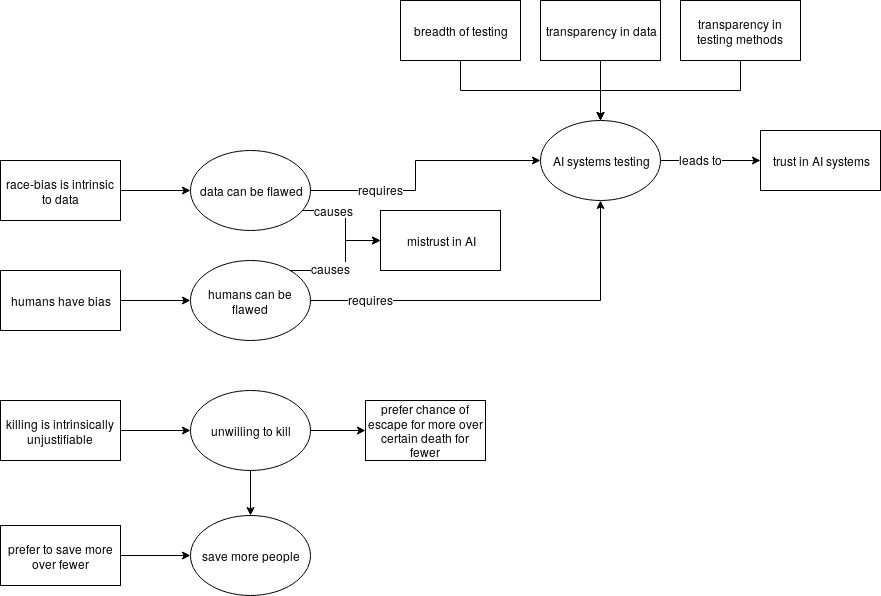
\includegraphics[scale=0.46]{figures/moral_ai_survey_analysis.jpg}
    \caption[]{Qualitative analysis of the survey results.}
    \label{fig:survey_analysis}
\end{figure}

% 
% test 40-60 100-0 0-100
% 

\begin{figure}[h]
    \centering
    \centerline{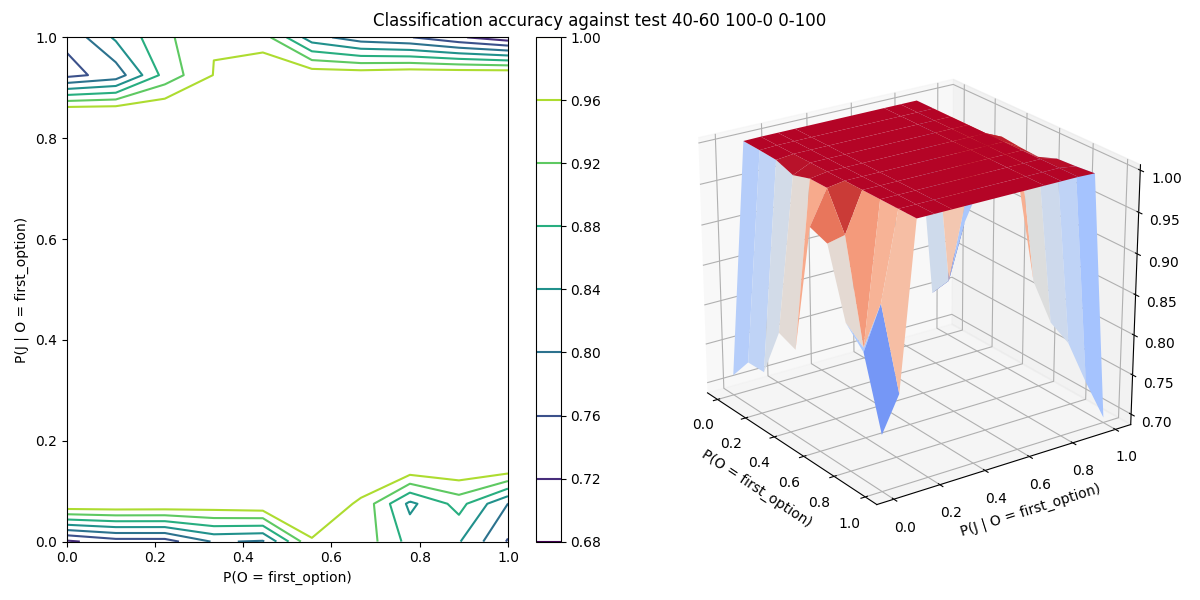
\includegraphics[scale=0.55]{test_40-60_100-0_0-100_accuracy.png}}
    \caption[]{The classification accuracy against \code{test 40-60 100-0 0-100}.}
    \label{fig:test_40-60_100-0_0-100_accuracy_plot}
\end{figure}

\begin{figure}[h]
    \centering
    \centerline{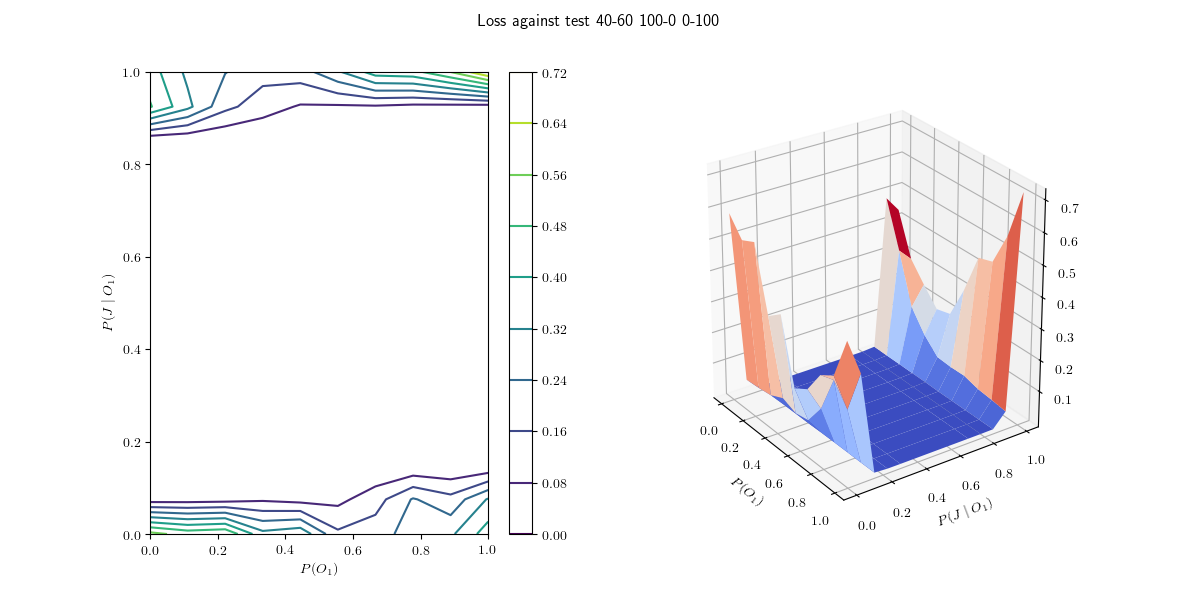
\includegraphics[scale=0.55]{test_40-60_100-0_0-100_loss.png}}
    \caption[]{The loss against \code{test 40-60 100-0 0-100}.}
    \label{fig:test_40-60_100-0_0-100_loss_plot}
\end{figure}

\begin{figure}[h]
    \centering
    \centerline{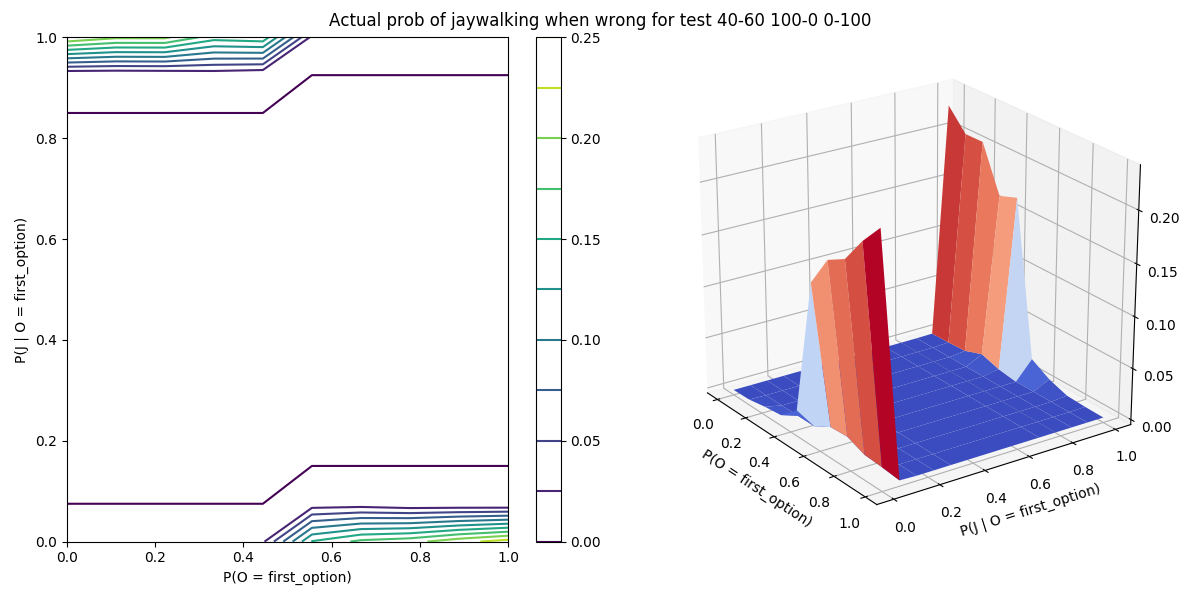
\includegraphics[scale=0.55]{test_40-60_100-0_0-100_jay_prob.png}}
    \caption[]{The actual jaywalking probability when classified incorrectly against \code{test 40-60 100-0 0-100}.}
    \label{fig:test_40-60_100-0_0-100_jay_prob_plot}
\end{figure}

% 
% test 40-60 0-100 100-0
% 

\begin{figure}[h]
    \centering
    \centerline{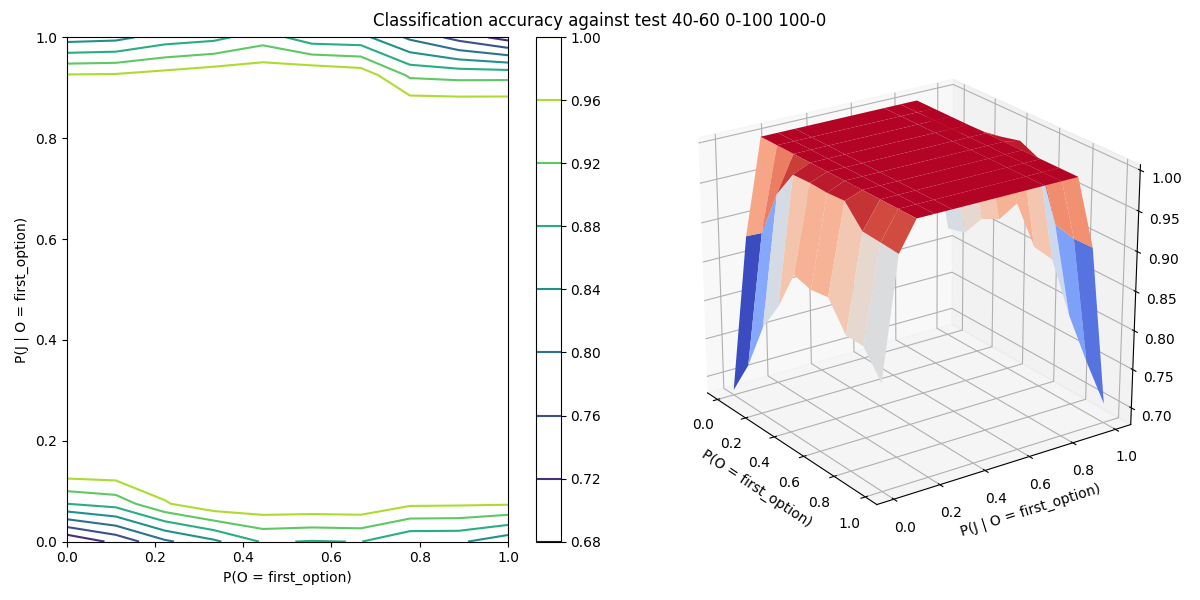
\includegraphics[scale=0.55]{test_40-60_0-100_100-0_accuracy.png}}
    \caption[]{The classification accuracy against \code{test 40-60 0-100 100-0}.}
    \label{fig:test_40-60_0-100_100-0_accuracy_plot}
\end{figure}

\begin{figure}[h]
    \centering
    \centerline{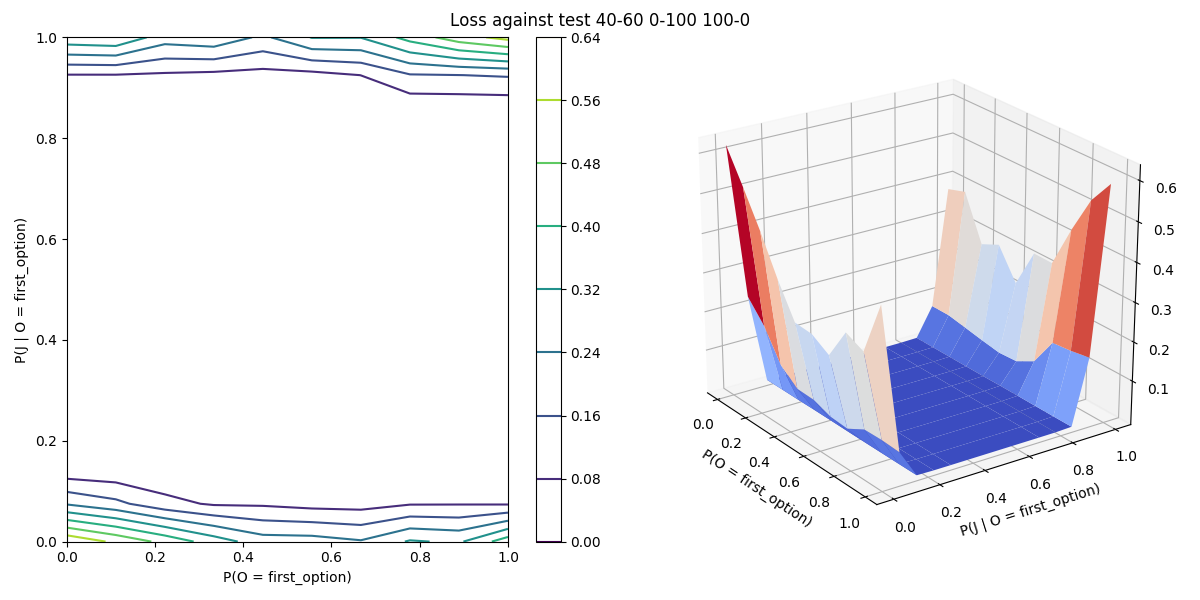
\includegraphics[scale=0.55]{test_40-60_0-100_100-0_loss.png}}
    \caption[]{The loss against \code{test 40-60 0-100 100-0}.}
    \label{fig:test_40-60_0-100_100-0_loss_plot}
\end{figure}

\begin{figure}[h]
    \centering
    \centerline{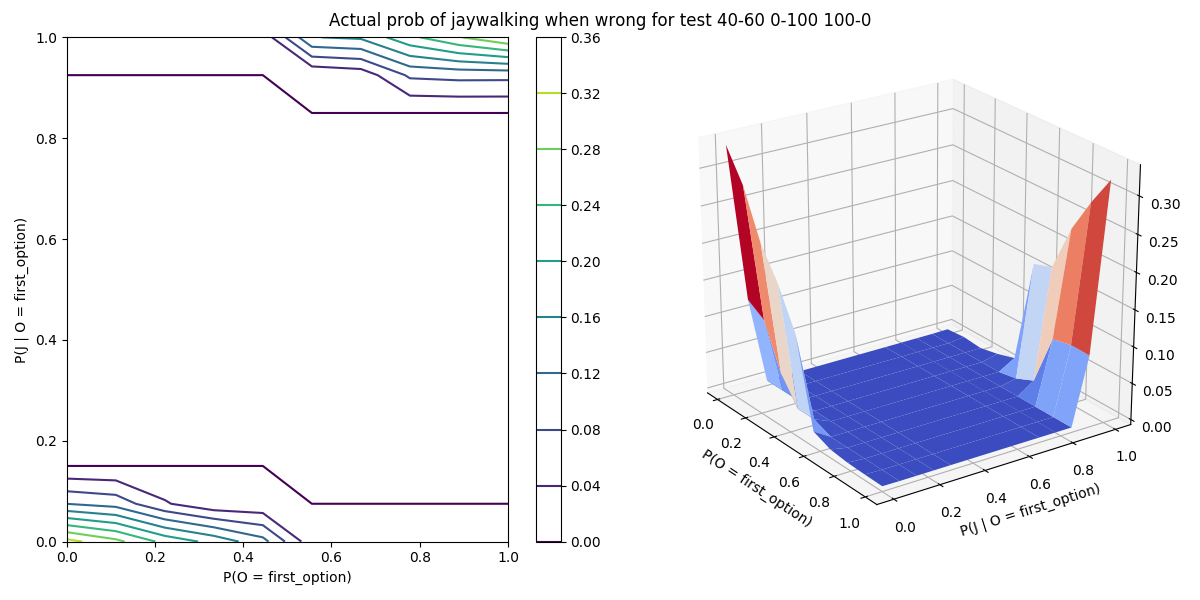
\includegraphics[scale=0.55]{test_40-60_0-100_100-0_jay_prob.png}}
    \caption[]{The actual jaywalking probability when classified incorrectly against \code{test 40-60 0-100 100-0}.}
    \label{fig:test_40-60_0-100_100-0_jay_prob_plot}
\end{figure}

% 
% test 40-60 80-20 20-80
% 

\begin{figure}[h]
    \centering
    \centerline{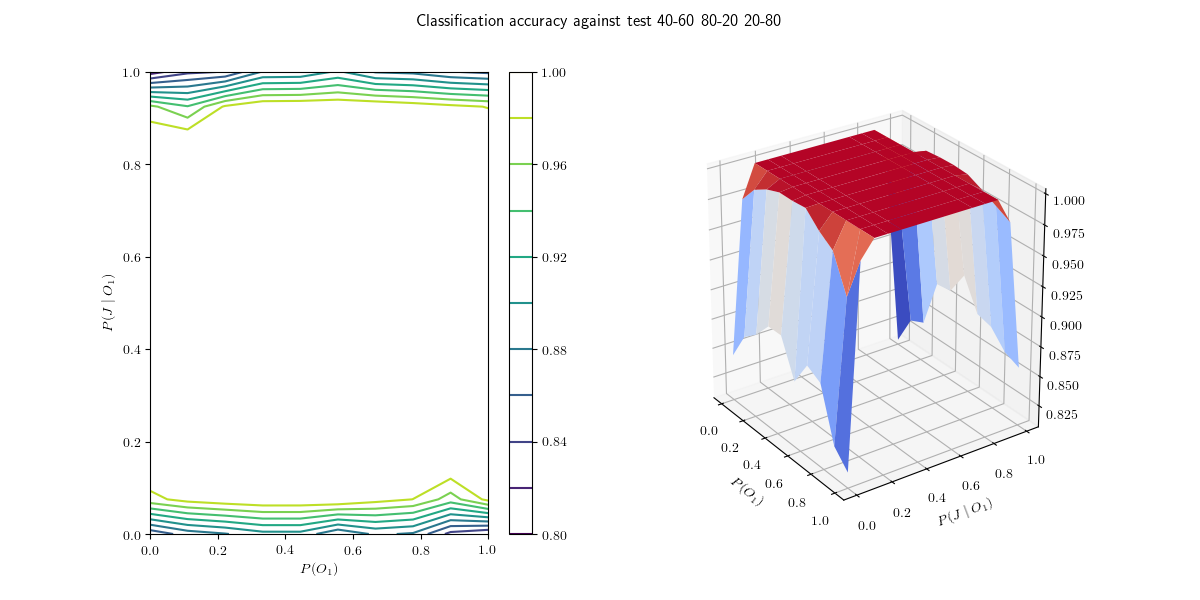
\includegraphics[scale=0.55]{test_40-60_80-20_20-80_accuracy.png}}
    \caption[]{The classification accuracy against \code{test 40-60 80-20 20-80}.}
    \label{fig:test_40-60_80-20_20-80_accuracy_plot}
\end{figure}

\begin{figure}[h]
    \centering
    \centerline{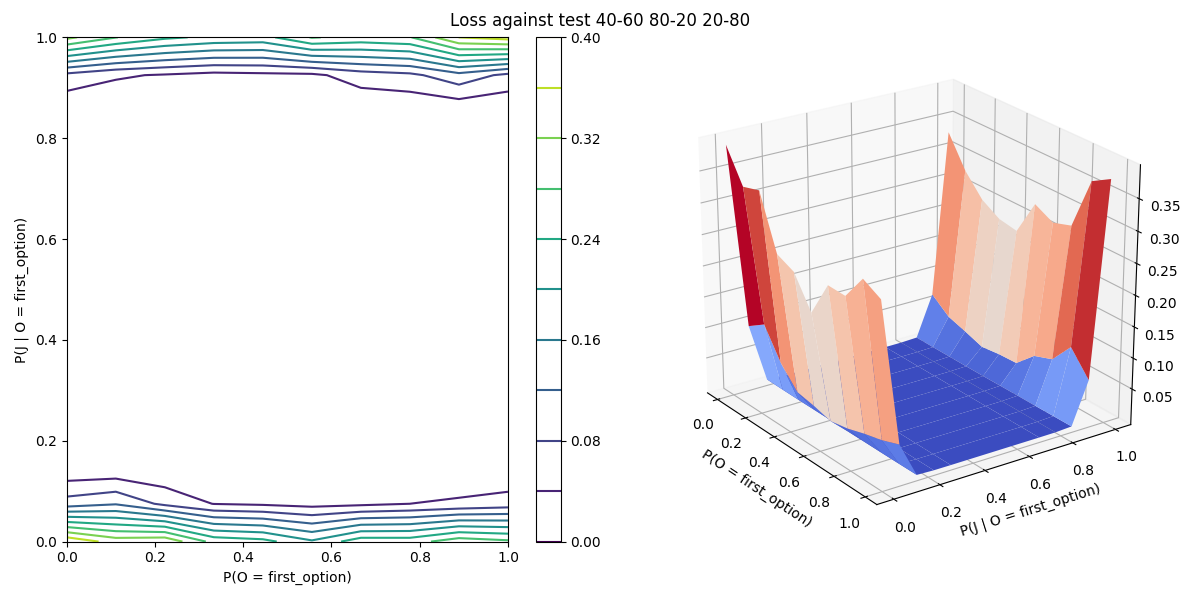
\includegraphics[scale=0.55]{test_40-60_80-20_20-80_loss.png}}
    \caption[]{The loss against \code{test 40-60 80-20 20-80}.}
    \label{fig:test_40-60_80-20_20-80_loss_plot}
\end{figure}

\begin{figure}[h]
    \centering
    \centerline{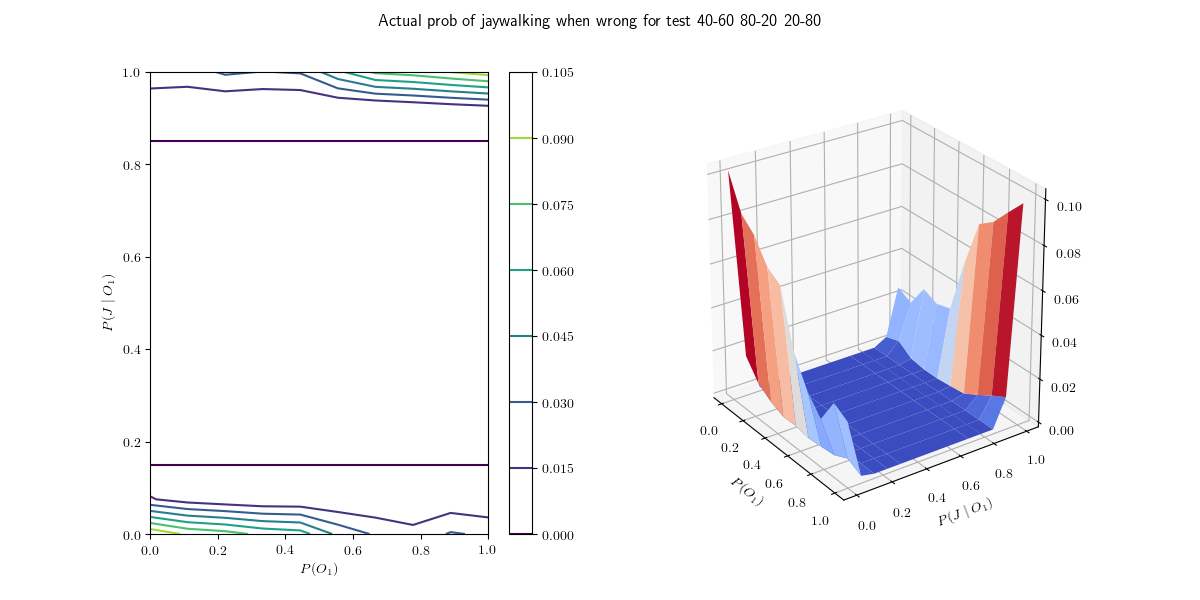
\includegraphics[scale=0.55]{test_40-60_80-20_20-80_jay_prob.png}}
    \caption[]{The actual jaywalking probability when classified incorrectly against \code{test 40-60 80-20 20-80}.}
    \label{fig:test_40-60_80-20_20-80_jay_prob_plot}
\end{figure}

% 
% test 40-60 20-80 80-20
% 

\begin{figure}[h]
    \centering
    \centerline{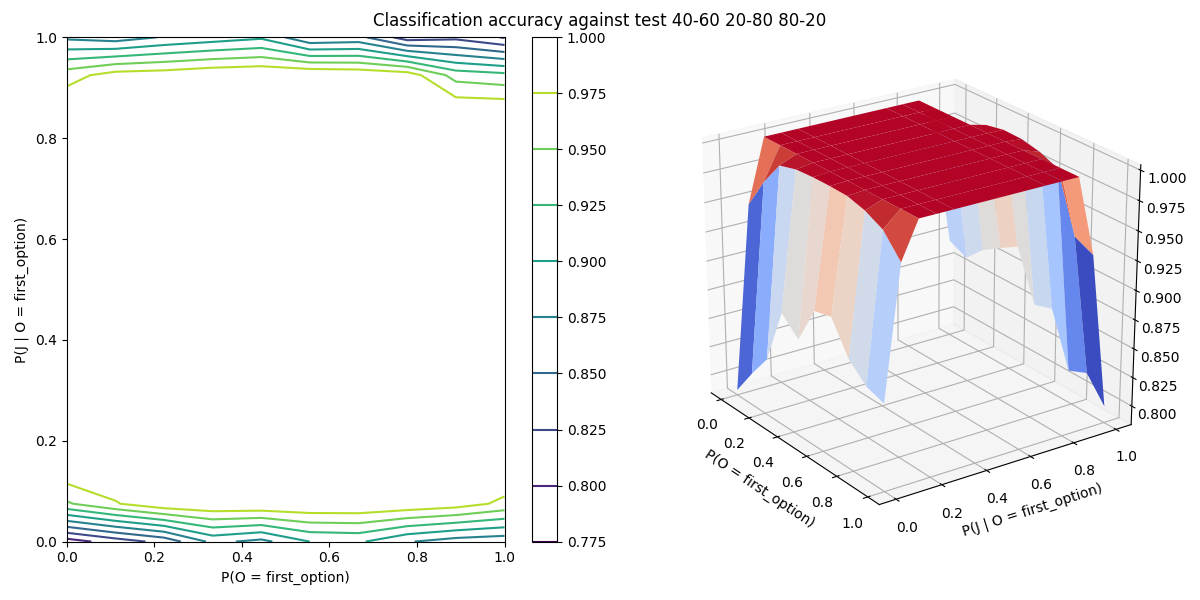
\includegraphics[scale=0.55]{test_40-60_20-80_80-20_accuracy.png}}
    \caption[]{The classification accuracy against \code{test 40-60 20-80 80-20}.}
    \label{fig:test_40-60_20-80_80-20_accuracy_plot}
\end{figure}

\begin{figure}[h]
    \centering
    \centerline{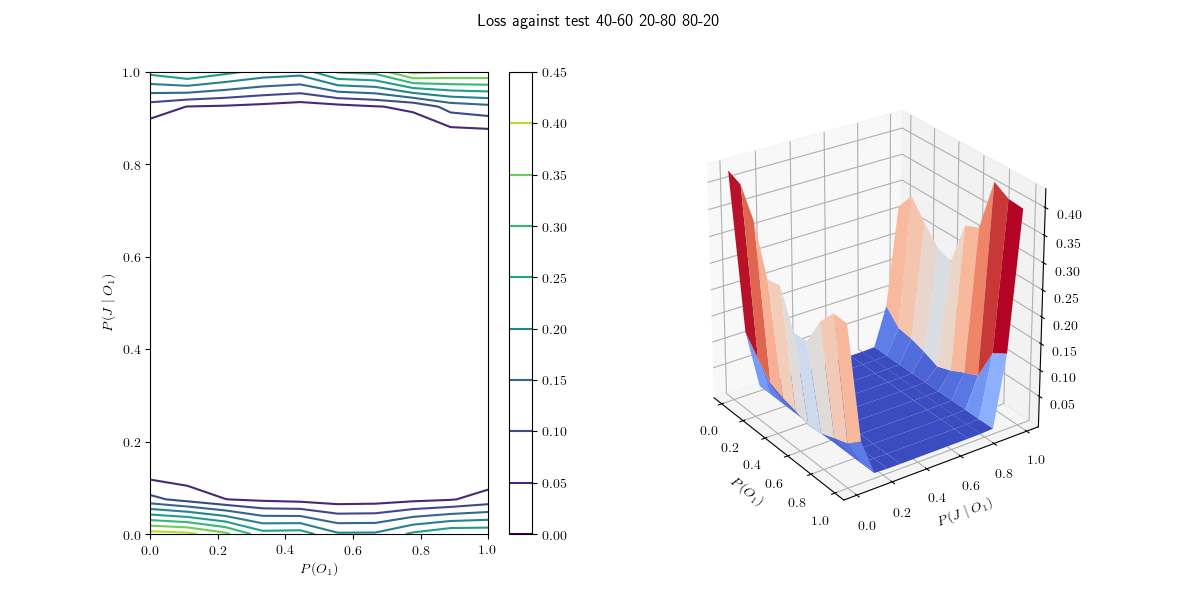
\includegraphics[scale=0.55]{test_40-60_20-80_80-20_loss.png}}
    \caption[]{The loss against \code{test 40-60 20-80 80-20}.}
    \label{fig:test_40-60_20-80_80-20_loss_plot}
\end{figure}

\begin{figure}[h]
    \centering
    \centerline{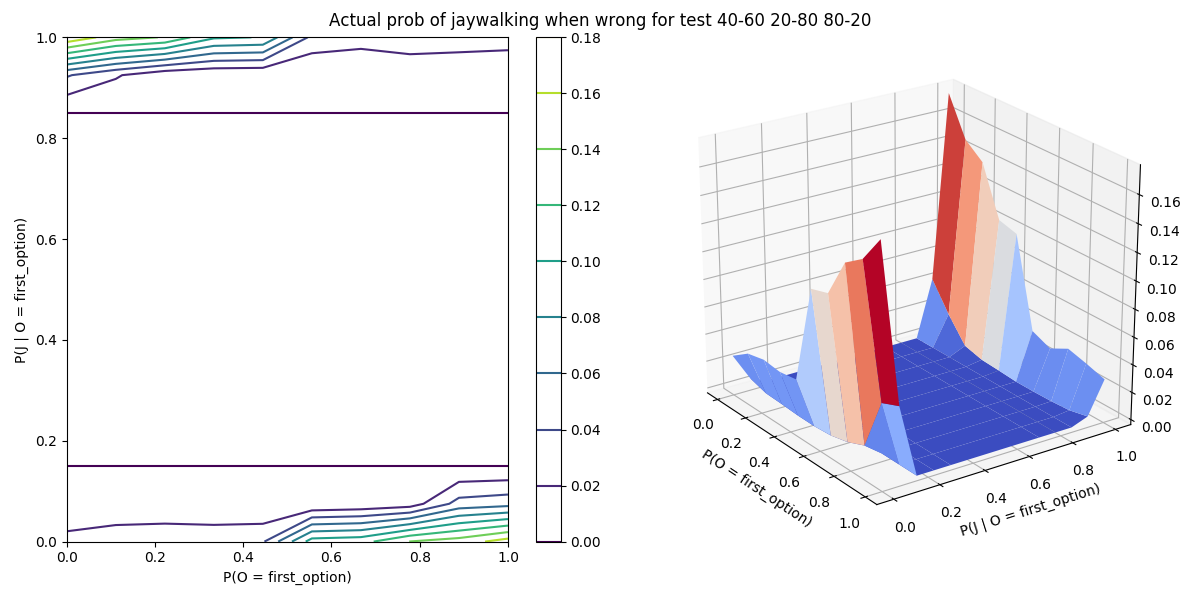
\includegraphics[scale=0.55]{test_40-60_20-80_80-20_jay_prob.png}}
    \caption[]{The actual jaywalking probability when classified incorrectly against \code{test 40-60 20-80 80-20}.}
    \label{fig:test_40-60_20-80_80-20_jay_prob_plot}
\end{figure}

% 
% test 50-50 50-50 50-50
% 

\begin{figure}[h]
    \centering
    \centerline{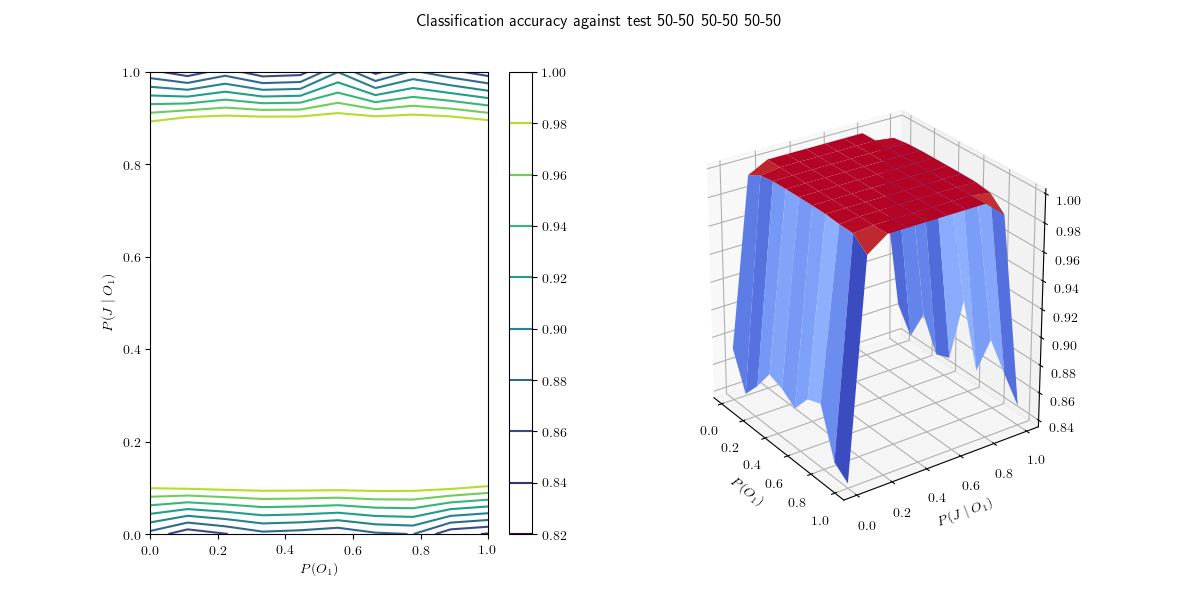
\includegraphics[scale=0.55]{test_50-50_50-50_50-50_accuracy.png}}
    \caption[]{The classification accuracy against \code{test 50-50 50-50 50-50}.}
    \label{fig:test_50-50_50-50_50-50_accuracy_plot}
\end{figure}

\begin{figure}[h]
    \centering
    \centerline{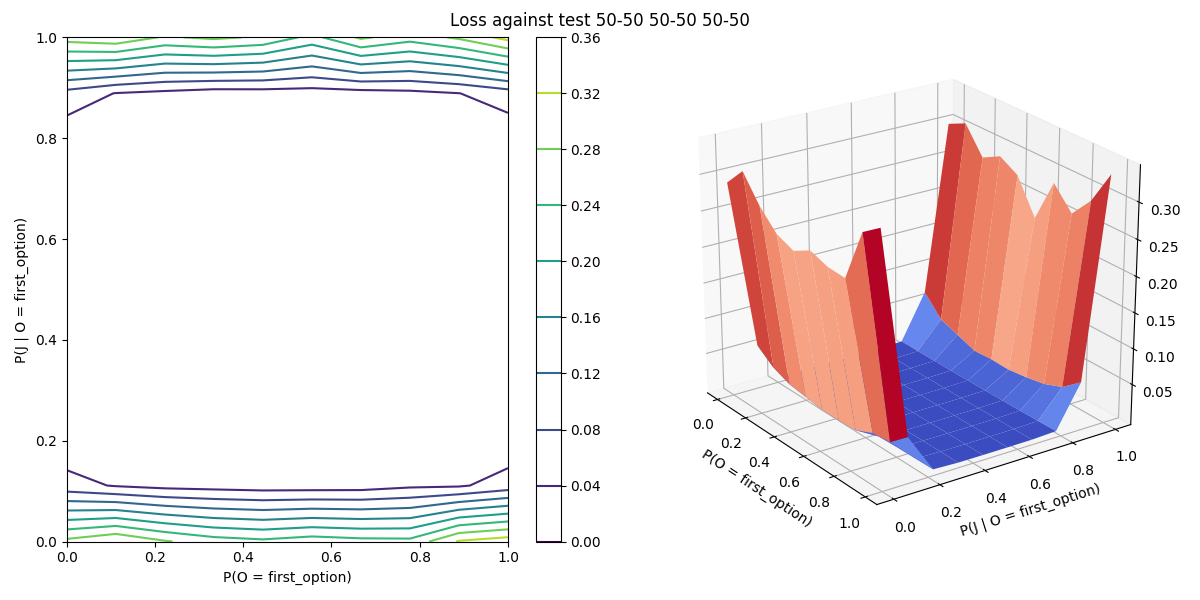
\includegraphics[scale=0.55]{test_50-50_50-50_50-50_loss.png}}
    \caption[]{The loss against \code{test 50-50 50-50 50-50}.}
    \label{fig:test_50-50_50-50_50-50_loss_plot}
\end{figure}

\begin{figure}[h]
    \centering
    \centerline{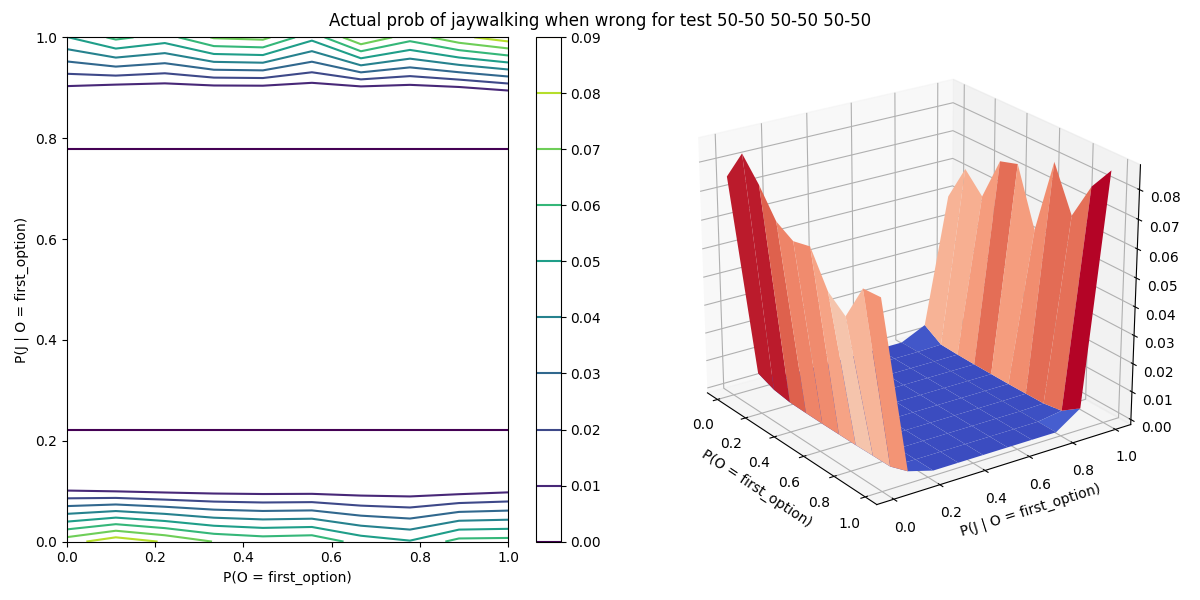
\includegraphics[scale=0.55]{test_50-50_50-50_50-50_jay_prob.png}}
    \caption[]{The actual jaywalking probability when classified incorrectly against \code{test 50-50 50-50 50-50}.}
    \label{fig:test_50-50_50-50_50-50_jay_prob_plot}
\end{figure}

\end{document}
